\documentclass[12pt]{article}

\title{ECE4063 - Image Thresholding}
%\subtitle{Progress Report}
\author{Emmanuel Jacyna - 24227498 \and James Anastasiou - xxxxxxxx}
\date{\today}

\usepackage[T1]{fontenc}
\usepackage[utf8]{inputenc}

\usepackage{graphicx}
\usepackage{tabularx}
\usepackage{float}
\usepackage{amsmath}
\usepackage{listings}
\bibliographystyle{unsrt}


\begin{document}
\pagestyle{myheadings}
  \maketitle
  \tableofcontents
  
  \section{Assumptions}
  
  \section{Documentation}
  \subsection{RGB to Grayscale conversion}
  
  \subsection{Histogram Module}
  \subsubsection{Description}
  The histogram module was based on a design from an article found on the IEEE website. The biggest problem we had in our initial attempts to create a histogram module as the latency in RAM access. The issue is that one cannot simultaneously read and write to a RAM, so when consecutive grayscale input values are identical, we are unable to correctly update the relevant RAM address. Our design overcomes this problem by specifically addressing the RAM latency issue. This histogram design consists of individual histogram \textit{cells}, each of which accesses its own RAM. By switching between these cells, the histogram is able to share the latency burden across multiple RAMs. Our histogram cells had a latency of three cycles, so we used three cells. This means that each cycle, one histogram cell is always ready to take in an input value. In order to get data out, we simply used a combinational logic block to address all three RAMs simultaneously and sum their outputs to get the true histogram value. Whilst this architecture does use more RAM resources, it is much easier to understand and thus enabled us to be confident that the system worked correctly.
  \subsubsection{RTL Diagram}
  \begin{figure}[H]
    \centering{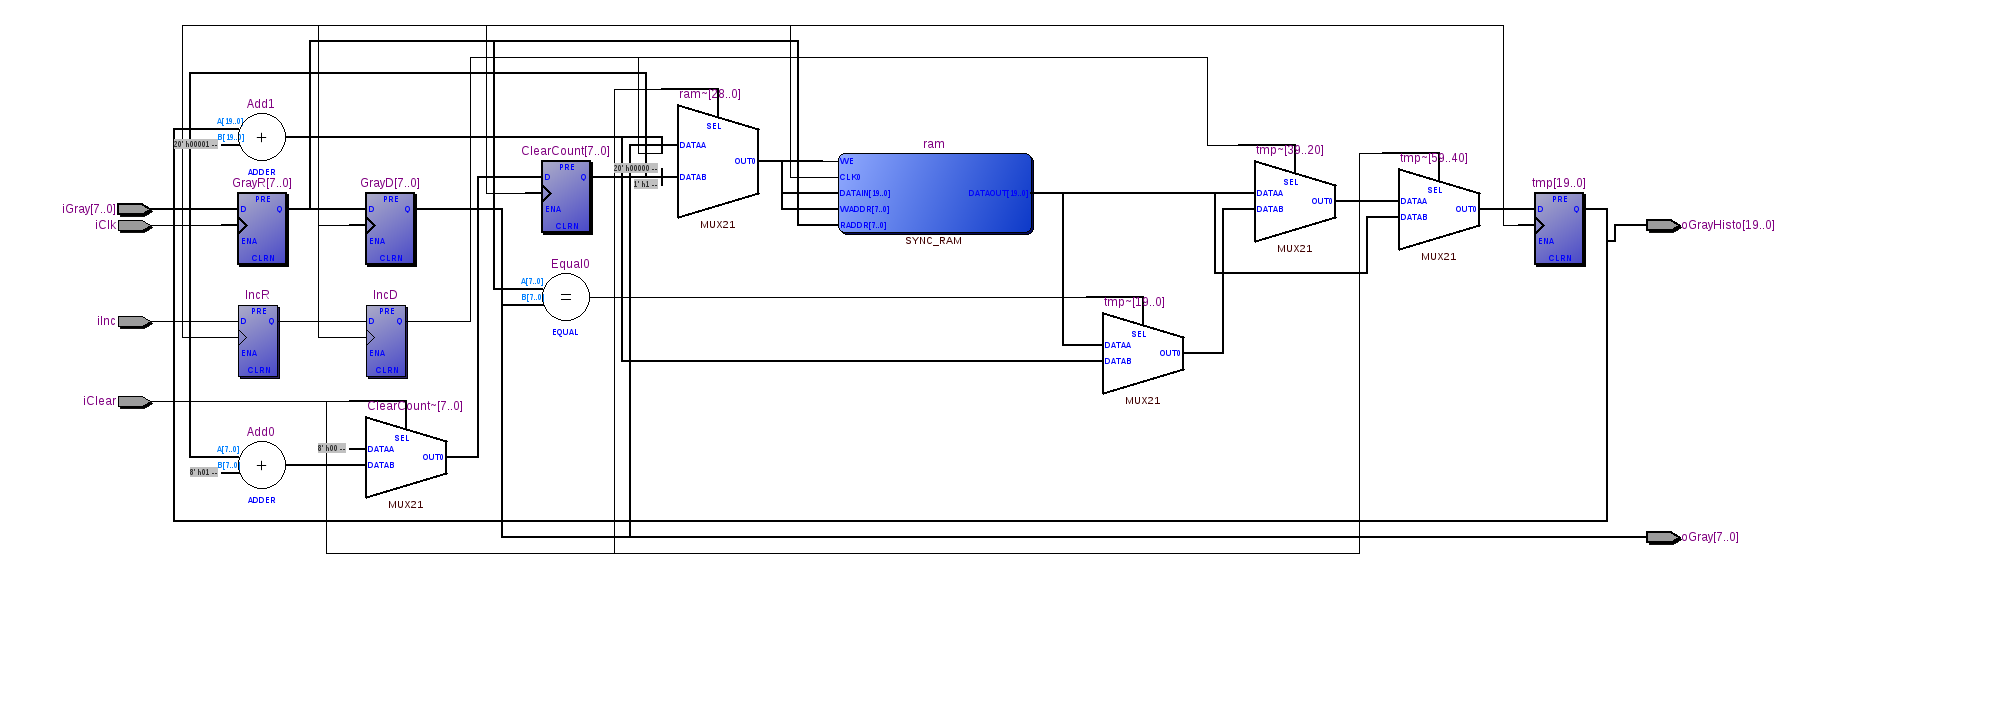
\includegraphics[scale=.8]{Images/HistogramRTL.png}}
    \caption{Histogram module RTL}
    \label{fig:histogram_rtl}
  \end{figure}
  
  \begin{figure}[H]
    \centering{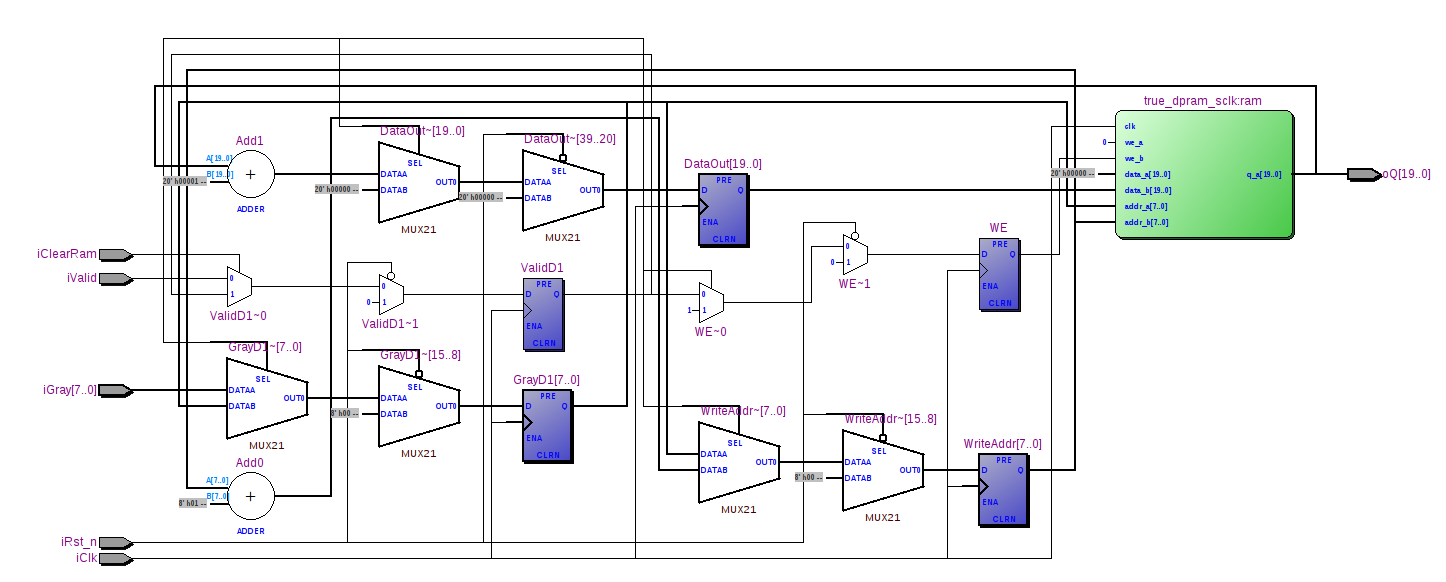
\includegraphics[scale=.8]{Images/HistogramCellRTL.png}}
    \caption{Histogram Cell module RTL}
    \label{fig:histogram_cell_rtl}
  \end{figure}
  
  
  \subsubsection{Module Testbench Results}
  
  \subsection{Cumulative Histogram Module}
  
  \subsection{Thresholding Module}
  \subsubsection{Description}
  The thresholding module is very simple. All it needs to do is take in an 8 bit greyscale value and output either a white (255) if the value is above the threshold, or a black (0) if the value is below the threshold. This is accomplished by hooking up a comparator to a multiplexer.
  
  \subsubsection{RTL Diagram}
  \begin{figure}[H]
    \centering{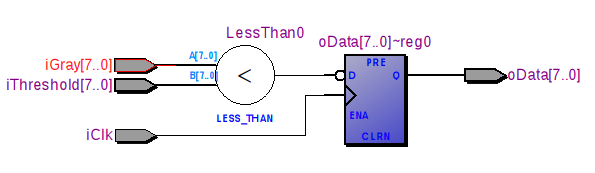
\includegraphics[scale=.8]{Images/ThresholderRTL.png}}
    \caption{Thresholding module RTL}
    \label{fig:thresholder_rtl}
  \end{figure}
  
  
  \subsection{Displaying things}
  \subsubsection{Description}
  In order to display the greyscale image, histogram, cumulative histogram, and thresholded image, we wrote a module to handle multiplexing between them using the switches on the DE2 board, called Arbitrator. This module takes in pixel outputs from the various modules and multiplexes them depending on the switch positions. In order to display images, we simply piggyback on the \(X\_Cont\) and \(Y\_Cont\) signals and modify the \(wr1\_data\) and \(wr2\_data\) inputs to the SDRAM with the appropriate pixel data. \\
      
  Displaying the actual histogram data requires slightly more effort. First we need to extract the histogram data from the histogram RAM and convert the histogram bin sizes into pixels for display on the screen. To do this we have a module called HistogramDisplayer. This module takes in the \(Y\_Cont\) signal and uses it to index the histogram RAM. Based on the histogram value from the RAM, it scales the histogram value, and uses the \(X\_Cont\) signal to determine the length of the line to be displayed. 
  
  \section{Acknowledgements}
  
  \section{Improvements}
  
  \section{Conclusion}
  
  
  
  
\end{document}
